%!TEX root = ../template.tex
%%%%%%%%%%%%%%%%%%%%%%%%%%%%%%%%%%%%%%%%%%%%%%%%%%%%%%%%%%%%%%%%%%%%
%% chapter3.tex
%% NOVA thesis document file
%%
%% Chapter with a short latex tutorial and examples
%%%%%%%%%%%%%%%%%%%%%%%%%%%%%%%%%%%%%%%%%%%%%%%%%%%%%%%%%%%%%%%%%%%%

\typeout{NT FILE chapter3.tex}%

\chapter{Architecture}
\label{cha:architecture}

In this chapter there will be a presentation of the architecture of the proposed solution as well as some insights into its 
implementation.

\section{System Overview}
\label{sec:systemoverview}
\paragraph{}The proposed solution is designed to address the complexities of navigating a 
tractor-trailer system in narrow environments, such as agricultural fields. This system integrates 
advanced path planning and control strategies to ensure safe practices, with collision avoidance, and 
effective navigation, tending to the specific needs of this type of system.

The system is divided into two main components: a self-propelled tractor and a non-propelled trailer. 
The tractor is an Agilex Scout which is a four-wheeled differential driven robot that serves as the 
navigation unit. The trailer, designed for modularity can have its own independent functionalities 
allowing for a simpler maintenance and adaptability to different tasks. This modullarity allows 
for the independant development of the tractor's navigation and control systems without the need knowledge of the trailer's 
payload or functionalities, with perhaps the exception of the trailer hindering the sensor's view 
or the trailer's weight exceeding the tractor's capabilities.

The solution proposed in this work is divided into four main modules:
\begin{itemize}
    \item \textbf{Environment}: This module is responsible for the representation of the real world, or actually be the real world. This is where the robot will operate.
    \item \textbf{Sensor perception}: This module is responsible for gathering data from the environment and converting it into usable information like localization and estimation.
    \item \textbf{Path planning}: This module is responsible for generating a feasible path from the current position to the desired goal.
    \item \textbf{Control}: This module is responsible for tracking the generated path and ensuring the tractor-trailer system follows it safely without collisions.
\end{itemize}

The overall functioning of the system is as follows: the tractor is at a point in the environment, simulation or real world, 
the user then requests a movement to a specific position, the path planning module will then generate a path from the current 
position, estimated with sensor gathered data, to the desired goal. The path is then forwarded to the 
controller which will then track it by computing the necessary angular and linear velocities while ensuring the 
physical constraints of the tractor-trailer system a re respected.
 

% insert figure with an uml diagram of the syste architecture

\section{Hardware}
\label{sec:hardware}

\paragraph{}The tractor used is an Agilex Scout which is a four wheeled differential driven robot, 
equipped with a NVIDIA Jetson Agx Xavier as the main computer, a LIDAR, an \gls{IMU} and wheel decoders. The Lidar is 
used to get a point cloud of the robot's surroundings, this point cloud is then fed 
into the localization algorithm to convert it into a laserscan and be used to help get 
the robot's position relatiive to the world. Thsi can only be achieved if there is 
a previously built map of the environment, which is done using the \gls{SLAM} algorithm. Along with 
the Lidar, the \gls{IMU} and wheel decoders are used to get the robot's accelerations in the three axes and the 
wheel's rotations respectively. All these sensors are fused together using an Extended Kalman Filter to get the robot's 
odometry.
 
\begin{figure}[h]
    \centering
    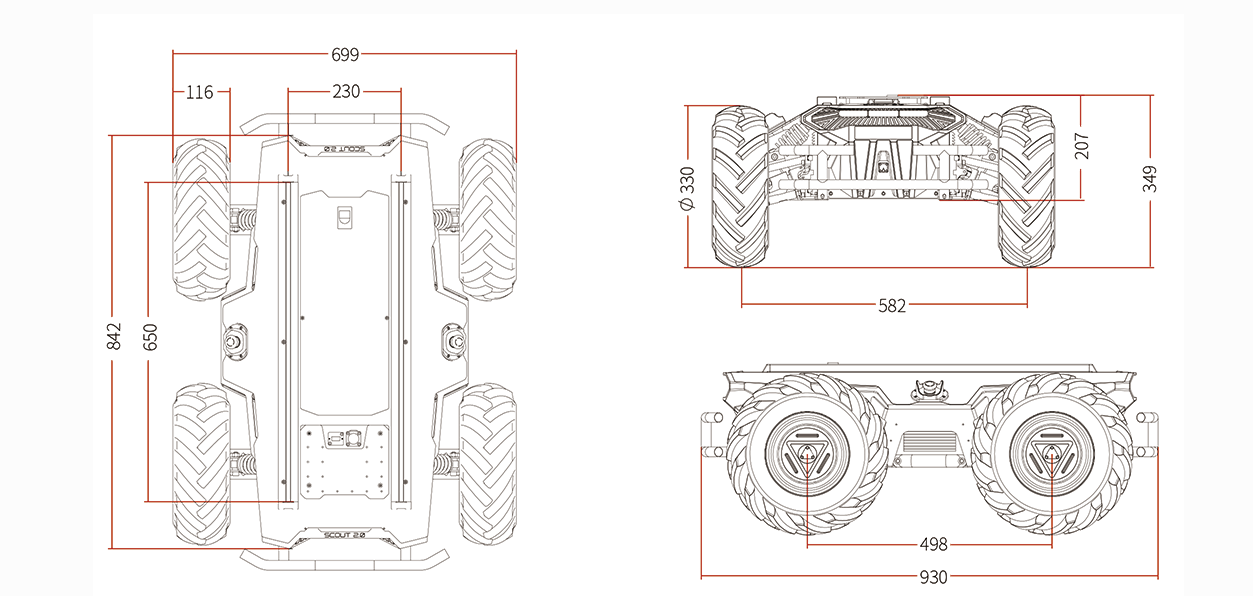
\includegraphics[width=0.9\textwidth]{tractordim.png}
    \caption{Agilex Scout dimensions.}
\end{figure}

The previous figure only sows the robot and its dimensions, however, the 
tractor is equipped with an additional rack, at the top, where the computer, Lidar and all other required electronics 
are mounted.
% \begin{figure}[h]
% \centering
% \includegraphics[width=0.9\textwidth]{tractorack.png}
% \caption{Rack with the main computer and additional eletronics.}
% \end{figure}
Additionally, the tractor is pulling a trailer, which is equipped with 
a spray system, however for the sake if simplicity, to thest the navigation 
and control algorithms, the tests were be done with the following trailer:
\clearpage
\begin{figure}[h]
    \centering
    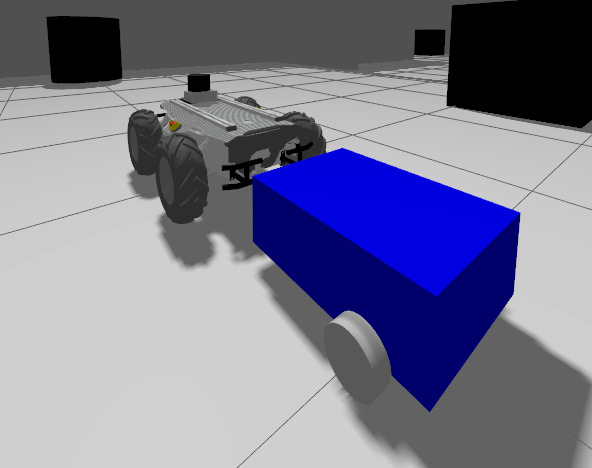
\includegraphics[width=0.9\textwidth]{trailergazebo.jpg}
    \caption{Tractor-trailer system simulated in Gazebo Classic.}
\end{figure}

The trailer shown in the figure above, is a representation of a generic trailer, not having any specific 
functions other than follwoing the systems dynamics, which is the main focus of this work.
% \begin{figure}[h]
% \centering
% \includegraphics[width=0.9\textwidth]{trailerdim.jpg}
% \caption{Tractor-trailer system simulated in Gazebo Classic.}
% \end{figure}

\section{Planner}
\label{sec:planner1}
The planner is a Voronoi Hybrid A* mixeture which takes the 
ability to generate feasible paths from the Hybrid A* and the 
added velocity of having a pre-computed Voronoi graph to expand 
from.

The following flowchart shows the logic of the planner, starting with 
the request for movement, assigning a goal target. Then, the planner will 
preform a A* search on the Voronoi Graph, starting from the current robot 
positon, to the goal pose. The A* search will return a path which consists 
of a series of subgoals which will later on be used to speed up the 
path creation process. Having the subgoals, the next step is to try and 
find a feasible path from the current position to the subgoal nearest to 
the goal pose, in this case, since it is the first iteration, the actual goal. 
If the path is feasible, then the planner will simply return said path, otherwise
 the planner will try to do the same but with the next subgoal, until it either finds 
a feasible path or exhausts all the subgoals. If it finds a path, it will 
repeat the previous process, but instead of using the current position as the 
starting configuration, it will use the subgoal which a path was able to be 
computed to. If it exhausts all the subgoals, then it will try and compute a new node, 
a Hybrid A* node, which consists of a segment, starting from the current algorithmic position 
(can be the start point or a subgoal depending if a path was found previously), to any point 
that is reachable by the tractor at a distance $d$ defined by the user, and then assign them as the 
current algorithmic position to run the Dubins loop again.
\begin{figure}[h]
    \centering
    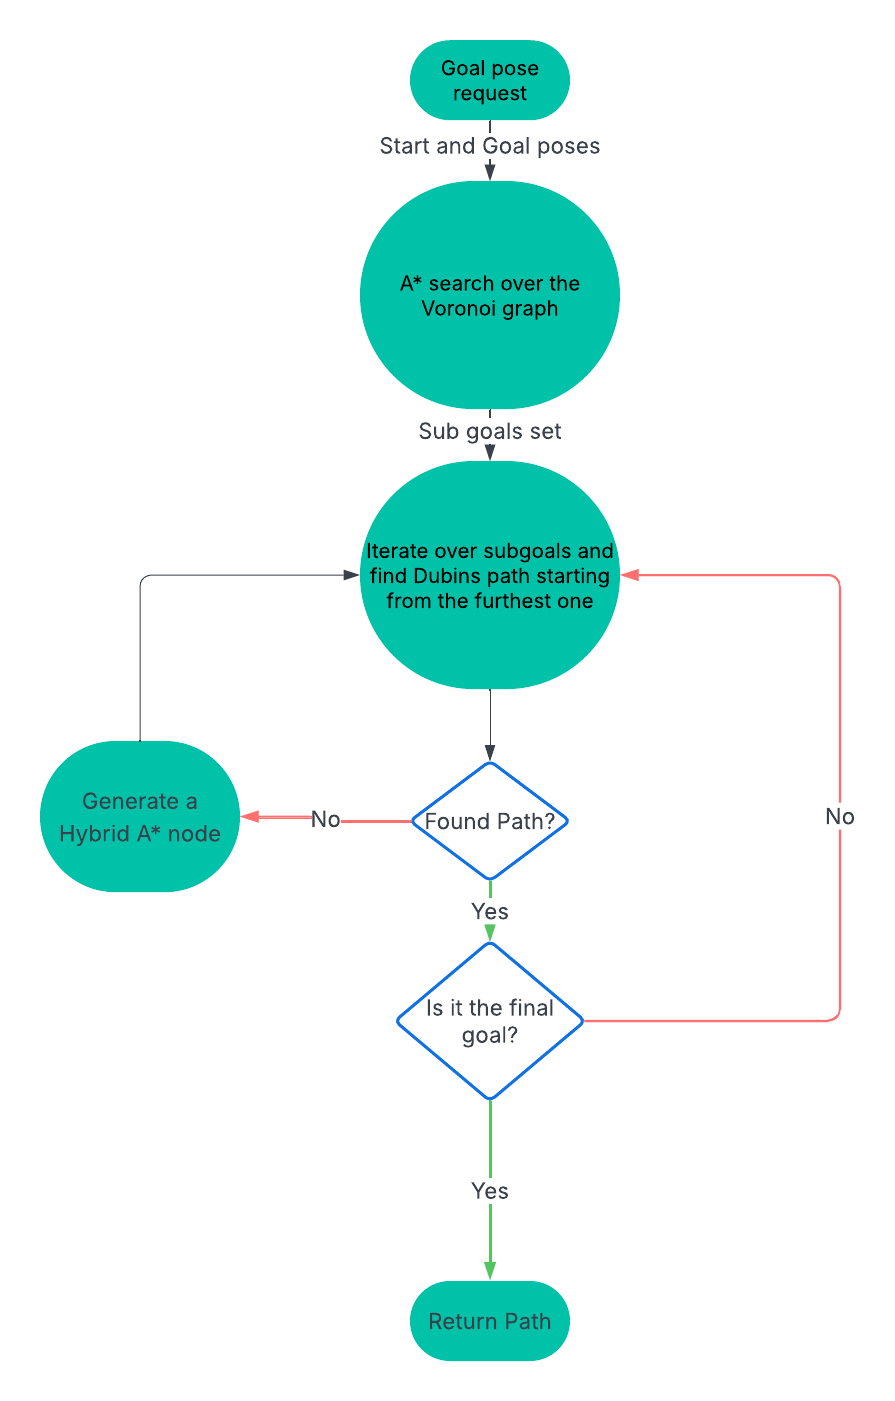
\includegraphics[width=0.80\textwidth]{Flowchart.png}
    \caption{Planner logic flowchart}
\end{figure}
\clearpage
\begin{figure}[h]
    \centering
    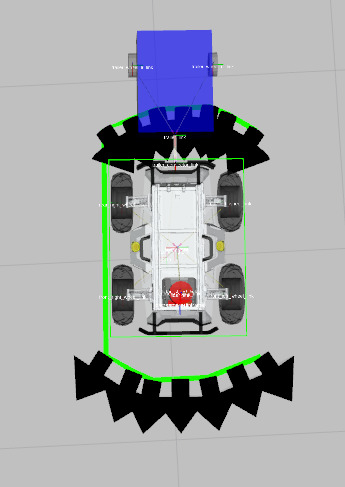
\includegraphics[width=0.6\textwidth]{Hybridastararrows.jpg}
    \caption{New Hybrid A* nodes, in black.}
\end{figure}

\section{Controller}
\label{sec:controller}
A path is nothing if it cannot be followed so, a controller capable of 
attending to this system's needs is required. This controller will 
receive as input the generated path by the planner and will try to track it. 
This is achieved in two steps, first, having the current positions in mind, 
it will choose the next subgoal in the path. Since the controller is 
a \gls{PP} controller, the subgoal is chosen depending on the lookahead distance, 
as explained in \ref{subsec:PP}. The next step is to compute the angular velocity needed 
for the robot to reach said subgoal. For this, two controllers were used:
\begin{itemize}
    \item \textbf{Forwards Controller}: Used when the tractor is moving forwards.
    \item \textbf{Backwards Controller}: Used when the tractor is moving backwards.
\end{itemize}
The choice of controller depends on the orientation of the tractor and 
direction to the next subgoal. The need for two controllers arises from 
the fact that when moving backwards, the movement needs to be optimised 
for the trailer's position and orientation, while when moving forwards, 
the movement needs only to be optimised for the tractor's movement as the 
trailer positions are move predictable when moving forwards.

The forwards controller is defined by the following equations:
\begin{equation}
    \omega = \tan^{-1}\left(\frac{2*WB*sin(\epsilon_{\theta_0})}{l_f}\right)
\end{equation}
where $WB$ is the wheelbase of the tractor, $l_f$ is the lookahead distance and 
$\epsilon_{\theta_0}$ is the error in the angle between the tractor and the next goal.
\begin{equation}
    \epsilon_{\theta_0} = \tan^{-1}\left(\frac{t_y - y_r}{t_x - x_r}\right) - \theta_0
\end{equation}
The $t_x$ and $t_y$ are target point coordinates and $x_r$ and $y_r$ are the current tractor center coordinates. 
As explained previously, this controller only cares about the tractor's 
configuration, which makes having a feasible path all the more important.

The backwards controller, on the other hand, is defined by the following equations:
\begin{equation}
    \omega = V \left(-k (\theta_1 - \alpha^*) - \frac{sin\theta_1}{RTR}\right)
\end{equation}
where $RTR$ is the distance between the hitch joint and the trailer's real axle, 
$k$ is a constant, $\theta_1$ is the angle between the tractor and the trailer, 
$V$ is the linear velocity of the tractor and 
\begin{equation}
    \alpha^* = tan^{-1}\left(\frac{2*RTR*sin(\epsilon_{\theta_1})}{l_f}\right)
\end{equation}
with
\begin{equation}
    \epsilon_{\theta_1} = \tan^{-1}\left(\frac{t_y - y_t}{t_x - x_t}\right) - \theta_t
\end{equation}
where $t_x$ and $t_y$ are the target point coordinates and $x_t$ and $y_t$ are the current trailer real axle coordinates and 
$\theta_t$ is the orientation of the trailer. It is observed that 
these equations are similar to the forwards controller, however, they differ 
in the fact that the goal pose is defined by the trailer's position. Even though 
this controller is taking the trailer's constraints into account, due to 
the inate nature of the tractor-trailer system being non-holonomic, the 
path planner is still the one responsible for maintaining the feasibility 
of the movement.


\section{Collision Avoidance}
\label{sec:collision}
The collision avoidance aspect of the controller is of the utmost importance 
in real world scenarios when dealing with possible workers in the field. To achieve 
this safety requirement the controller is equipped with a collision detector 
which will check for obstacles in the way of the tractor-trailer system and stop until the 
obstacle is no longer in the way or another path update has been sent.

The collision detection is done by checking if theres an obstacle between the 
tractor and its next goal in the path. If the robot is reversing, instead 
of checking the tractor's next goal, it will check the trailer's.

\section{System Overview}
\label{sec:systemoverview}
The system is a modular one, where every module is responsible for a 
specific task and toguether they form a complete system. 
